
\documentclass[conference]{acmsiggraph}

% for control over itemize
\usepackage{enumitem}

%to put the link to the video
\usepackage{url}
\usepackage{hyperref}

\TOGonlineid{45678}
\TOGvolume{0}
\TOGnumber{0}
\TOGarticleDOI{1111111.2222222}
\TOGprojectURL{}
\TOGvideoURL{}
\TOGdataURL{}
\TOGcodeURL{}

\title{Real-time gait control for partially immersed bipeds}
% *** Walk Motion Control in Partial Immersion - à décider à la fin ***

\author{paper ID}
%Soumission est double-blind, mettre l'ID du papier à la place (donné à la création de la soumission).
%Samuel Carensac\thanks{e-mail:samuel.carensac@gmail.com}, Nicolas Pronost, Saida Bouakaz\\University Claude Bernard Lyon 1, LIRIS
\pdfauthor{paper ID}

\keywords{Virtual Human, Physics-based animation, Motion control, Real-time liquid interaction, Offline optimization}

\begin{document}

\teaser{
   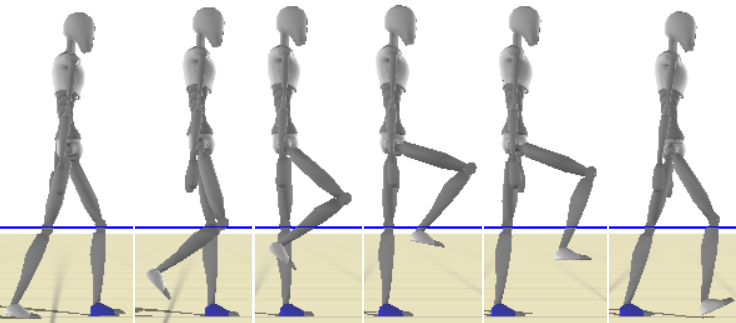
\includegraphics[height=1.5in]{images/3_6_1_50cm.png}
   \caption{Our controller allows the real-time simulation of a character walking while partially immersed. It demonstrates robust balancing, gait style adaptation to the environment and precise speed tracking. Here, the swing foot gets out of the water before the character starts moving forward. ***Not final image (need longer series)***}
	% *** Peut-être trouver une série où le pied sort complètement de l'eau ***
\label{fig:intro}
}

\maketitle

\begin{abstract}

Physics-based animation is an increasingly studied subject of computer animation because it allows natural interactions with the virtual environment. Though some existing motion controllers can handle the simulation of interactions between a character and a liquid, only few methods focus on the simulation of the locomotion of immersed bipeds. In this paper, we present a control strategy capable of simulating partially immersed gaits. The impact of the liquid on the character's motion is modeled through simple hydrodynamics. We design a controller allowing the combination of multiples gait styles, the conservation of balance through intelligent foot placement and precise control of the character's speed. We determine the optimal parameters for the controller by using an optimization process. This optimization is repeated for several scenarios where the character has to walk across a volume of liquid parametrized by its height. Our controller produces natural looking gaits while being capable of online adaptation to the variation of liquid height, to the modification of the liquid density and to the variation of the required character's speed.

\end{abstract}

\begin{CRcatlist}
  \CRcat{I.3.3}{Computer Graphics}{Three-Dimensional Graphics and Realism}{Animation}
\end{CRcatlist}

\keywordlist

%\copyrightspace

\section{Introduction}

Simulating realistic human motion is a key step in creating virtual environments. Over the years, these environments have become increasingly diverse and complex with a large number of elements that can influence the motion of a virtual character. In those cases, physics-based animation is preferred over kinematic animation since it does not need a series of exact position for each possible interaction. With this increasing complexity, it is difficult to achieve realistic interactions between animated characters and the environment using kinematics-based approaches. Physics-based animation uses physical phenomena (forces and torques) to manipulate the character. This allows the creation of a motion that will be directly impacted by the environment. A growing number of contributions are now working on building controllers using simulated physics~\cite{geijtenbeek2012interactive}. Although they inherently allow obtaining interactions with the environment, the manipulation of the character becomes more complex as no direct control over the position of the limbs of the animated characters is possible.

The main challenge of a controller is to allow high level parametrization of the system under the constraint of partial immersion. For example, these high level parameters may be the character's speed, the direction of displacement or the motion style. The need to simulate a large number of motion styles (walking, running, jumping...) makes creating a generic controller extremely challenging. Similarly, the mastery of multiples interactions with the environment also increases considerably the complexity of the system. This is why the existing controllers focus on the study of a limited number of motion styles at a time and interactions with the environment~\cite{geijtenbeek2012interactive}. We focused on the control of walking in partial immersion conditions in a liquid. Our objective was to define and implement the necessary mechanisms to a physics-based controller to allow real-time animation of a virtual character interacting with a liquid. Our controller is capable of great freedom of gait style and precise tracking of the character's motion speed.

The remainder of this paper section~\ref{sec:previous_works} reviews previous. Section~\ref{sec:overview} proposes an overview of our system. Sections ~\ref{sec:ext_forces}, ~\ref{sec:control_framework} and \ref{sec:optimisation} focuses on the techniques used in the implemented system. Section ~\ref{sec:implementation} presents the parameters used for our implementation. Section~\ref{sec:results} illustrates a variety of results, provides discutions and gives the limits of our method. Section~\ref{sec:conclusion} summarises our approach and highlightq future areas of work.
 
\section{Previous works}
\label{sec:previous_works}

%*** ajouter une second citation avec un autre état de l'art***
Numerous works on control of virtual characters with simulated physics can be found in the literature~\cite{geijtenbeek2012interactive}. Among those works, some share common characteristics with our objectives.

Our work share some features of the SIMBICON (SIMple BIped CONtroler)~\cite{yin2007simbicon} and associated works. Among them, \cite{coros2009robust} proposes a system integrating multiples controllers for navigation task. The drawback is that the system is designed to use optimization to determine how the different controllers should be used. To enable the use of low gains in the PD-controllers different methods have been used such as a feedforward system~\cite{yin2007simbicon} or the computation of torques to compensate the effect of gravity~\cite{coros2010generalized}.

\textbf{\textit{Balance control}} is one of the key systems in physics-based simulation. The original SIMBICON uses for instance secondary PD-controllers on the key joints (stance ankle and swing hip) to dynamically adapt the tracked positions. One way to compute a balance aware foot placement during walk motion is to use an Inverted Pendulum Model (IPM)~\cite{coros2010generalized,kajita20013d}. This model can be used to dynamically compute the trajectory of the swing foot but it limits the range of possible gaits styles.

\textbf{\textit{Velocity control}} is often one of the required characteristics of physics-based controllers. Some systems are capable of adapting to online variations of the desired velocity. In~\cite{coros2009robust} where multiple controllers are combined for specific motions as forward and backward walks. The IPM based systems offer an inherent control though imprecise as it does not consider the observed velocity~\cite{coros2010generalized}. The use of horizontal virtual forces has been a way to obtain a precise control of the speed and balance of the character~\cite{coros2010generalized,geijtenbeek2012simple}. This system is based on secondary PD-controllers to compute the requisite force. The static gains and constant used in those systems make them unable to track correctly the target velocity when the character is subject to a variable environment (e.g. apparition of a liquid medium). 

\textbf{\textit{Movement in liquids}} have been studied in both simulation~\cite{yang2004layered,si2014realistic} and biomechanics~\cite{barela2006biomechanical,chevutschi2009comparison}. Those works mainly focus on swimming control for simulation works and walk study with high level of immersion for biomechanics studies making them unusable in our scenarios. One can also mentions ~\cite{lentine2011creature} who simulating human walk under wind forces. Most of those works use the Navier-Stockes equations to simulate the liquids making them ineffective to obtain real-time and interactive simulations.

In this paper we propose a novel controller showing the following characteristics:
\begin{itemize}
\item{real-time interactive simulation by using simple hydrodynamics to simulate the impact of the liquid on the motion}
\item{dynamic gait style adaptation by combining multiple reference controllers}
\item{liquid aware gait styles by specific IPM usage and offline optimization}
\item{precise tracking of target velocity by using learning strategies}
\end{itemize}

\section{Overview}
\label{sec:overview}

\begin{figure}[t]
\centering
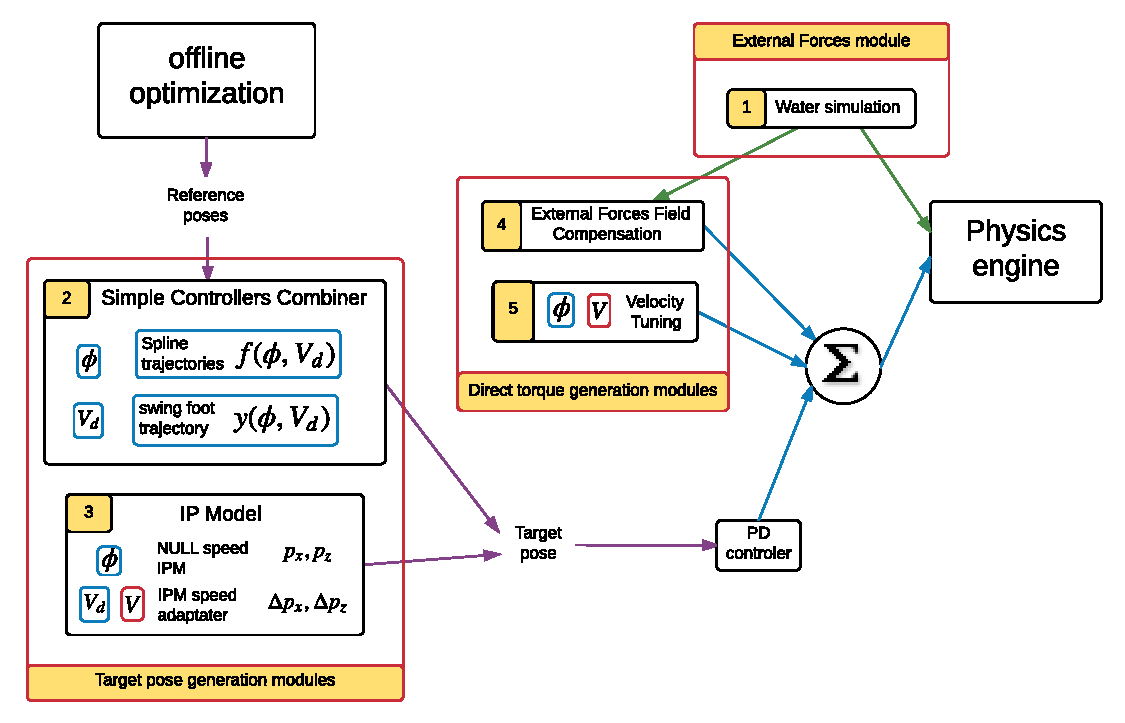
\includegraphics[scale=0.45]{images/general_process.pdf}
\caption{System overview. (1) influence of liquid through external forces; (2) a combination of controllers generating the target poses; (3) an IPM for predictive foot placement; (4) an external force-field compensation helping the PD-controller; (5) velocity tuning for fine corrections of velocity and balance.}
\label{fig:shema_controler}
\end{figure}

Our controller consists of five key components that are classified in three categories (figure \ref{fig:shema_controler}).

First we simulate the liquid impact on the character by applying external forces computed by simple hydrodynamics (drag, friction and buoyancy) allowing us to obtain real-time interactions between the liquid and the character (section~\ref{sec:ext_forces}). Our method combines various controllers, each one defining a gait style depending on the simulation conditions (e.g. liquid level, target speed) allowing an adaptive evolution of the gait style (section~\ref{sec:multi_state}). The specified trajectories for the joints composing the swing leg are overridden by the results of an IPM if the character is in the falling phase of a step or if the controller detects a loss of balance (section~\ref{sec:specific_ipm}).

We augment the PD-controller with torques computed through an external force-field compensation. Our system is a extension of Coros et al.'s gravity compensation mechanism~\cite{coros2010generalized} and compute a significant part of the necessary torques (section~\ref{sec:ext_force_comp}).

Our controller includes a precise tracking of the desired velocity through an adaptive offset on the swing foot position computed by the IPM (section~\ref{sec:ipm_alt}). Our system presents an improvement of Coros et al.'s fine-scale control~\cite{coros2010generalized} by considering the intra-step speed variation of the character to compute a more efficient virtual force (section~\ref{sec:speed_virt_force}).

Finally, we use offline optimization to generate the reference poses used by the controller combinator. This optimization defines a gait style specific to a given scenario (section~\ref{sec:optimisation}).

\section{External Forces}
\label{sec:ext_forces}

Beside the ground reaction forces, the external forces generated in our system are the forces related to the influence of the liquid on the character. These forces are based hydrodynamics laws by considering two types of forces. The first one is buoyancy. We use the well-known equation $F_{B}=-V_i \rho g$ with $V_i$ the immersed volume of the physics representation of the immersed object. The second type of forces is the parasitic drag. We restrict the considered physics phenomena to the form drag and the skin friction, modeling the resulting force $F_D$ using the following equation:
$$
F_D=\frac{1}{2} \rho v^2 A_n C_d \times \mu
$$
%***mettre les symboles dnas l'ordre ou ils sont trouvés dnas la formule***
where  $\rho$ the fluid density, $v$ the relative speed to the fluid, $A_n$ the cross sectional area and $C_d$ is the drag coefficient. Due to the complexity of dynamically computing $C_d$, we set it to 1.0 (average value for a man). $\mu$ is a coefficient representing the fluid viscosity allowing us a rough representation of the friction. The velocity varying through the limbs we use a finite elements decomposition of the surface of each limb and compute the parasitic drag for each element individually. Thus the computation of the cross sectional area $A_n$ and the immersion test are both directly realized on each element.

\section{Control Framework}
\label{sec:control_framework}

Our system is built on the version of SIMBICON presented in~\cite{coros2010generalized}. The trajectories for the ankles, pelvis, back and head are specified in the coordinate system of the character. This coordinate system is similar to the global one but the z-axis indicates the direction that the character is currently facing. The trajectories for the shoulders, elbows, toes and the knee of the stance leg are specified using each joint local coordinates. Unlike~\cite{coros2010generalized}, we allow manual specification of the swing foot trajectory. This specification is made in the local coordinate system of the swing hip.

\subsection{Simple Controllers Combiner}
\label{sec:multi_state}

The \textit{Simple Controllers Combiner} allows us to observe dynamic variations of the gait style depending on the conditions of the simulation (e.g. liquid level). The principle is to use multiple simple controllers that are specified for one set of conditions. For this work, we limit the conditions to the walking speed and the liquid level but the system could handle other specifications. Each simple controller defines the trajectories for the joints that exhibit significant variations from one standard controller. For example, our standard controller is a forward walking controller and as such it specifies that the heel hits the ground before the toes do. If we want to be able to walk backward we will have to specify a simple controller specifying that the toes hit the ground before the heel and affect it a negative sagittal speed. Our system differs from the one presented in~\cite{coros2009robust} by two characteristics. First, we do not require each individual controller to produce a stable motion. In our system the balance is acquired by the use of an IPM. Second, each individual controller only specifies the joints where the variation from the standard state is significant. On a more conceptual view, in our system, we just want to specify the variations of the gait and not the variations of control strategy. Also we do not require an optimization step to find the optimal combination of the simple controllers. When the character ends a step, the system will compute a new trajectory for each joint. To find those trajectories we use an interpolation following a square-law between the trajectories specified for the two nearest simple controllers. For example, if we use controllers defined only by their reference speeds, we will use the two controllers $f_1$ and $f_2$ defined for the speeds $V_1$ and $V_2$ that are the nearest from the desired speed $V_d$ respecting $V_1 < V_d < V_2$. If we cannot find two speeds respecting this rule we directly use the nearest simple controller. The following equation gives how the resulting trajectories $f$ are computed:
$$
f=f_1*(1-R)+f_2*R   \quad \textrm{with} \quad   R=\left( \frac{V_d-V_1}{V_2-V_1} \right) ^2
$$

\subsection{Inversed Pendulum Model}
\label{sec:IPM}

We use an \textit{Inversed Pendulum Model} (IPM) supposing constant leg size and zero desired velocity similar to the one used in~\cite{coros2010generalized}. We have modified this model to allow the specification of previously impossible gaits styles and to enable a better tracking of the user's desired velocity. 

\subsubsection{Specific IPM Usage}
\label{sec:specific_ipm}

Our idea to enable the specification of new gait style is that the IPM does not need to control the swing foot during the whole step. We only need to control the position of the swing foot when the character is in a falling state, meaning when the vertical speed of the center of mass is positive $V_{COM}>0$. During a step, the falling phase corresponds to the end of the step. So during the first part of the step we will use a user defined trajectory for the swing foot. This allows the observation of vertical movement of the swing foot without any horizontal movement, which was previously impossible. This kind of gait style is important in our scenarios as it is typical of a character trying to minimize the drag from moving in a liquid (Figure~\ref{fig:intro}).

\subsubsection{IPM Result alteration}
\label{sec:ipm_alt}

To have a partial control of the velocity, \cite{coros2010generalized} uses a linear modification of IPM results depending on the desired character velocity ($\Delta(x,z)=-\alpha V_d$). Unfortunately it only works properly near the velocity for which the linear factor has been optimized. In particular, this system cannot handle the transition from an environment with a fluid medium to an unconstrained one.

Our solution is to add a supplementary offset $\Delta(x,z)_i$ to the results of the IPM. This offset will be modified at the end of each step $s$ depending on the difference between the current character velocity and the desired velocity $\Delta(x,z)_s = \Delta(x,z)_{s-1}+\beta(V-V_d)$ with $\beta$ a positive constant. The swing foot position from the IP model $P_{IPM}(x,z)$ will therefore be modified as follows:
$$
P(x,z) = P_{IPM}(x,z) - \alpha V_d + \Delta(x,z)_s
$$ 

\subsection{External Force Fields Compensator}
\label{sec:ext_force_comp}

Our \textit{External Force Fields Compensator} is an extension of the gravity compensation proposed in~\cite{coros2010generalized}. The goal is to dynamically compute a part of the necessary torques at each joint thus permitting the use of lower gains in the main PD-controller. Using virtual forces opposing the external force fields affecting the character gives us a good estimation of these torques. The external forces that we consider are the weight $P=mg$ of each body part of the character and buoyancy $F_B=-\rho V_i$. We chose to ignore the liquid drag in the compensator because it would imply the use of many small forces (depending on the precision of the finite elements) which would be time consuming to compensate with our method. So the final virtual force applied to each body part is:
$$
F=-mg+\rho V_i
$$

\subsection{Velocity Tuning}
\label{sec:speed_virt_force}

\begin{figure*}[t]
\centering
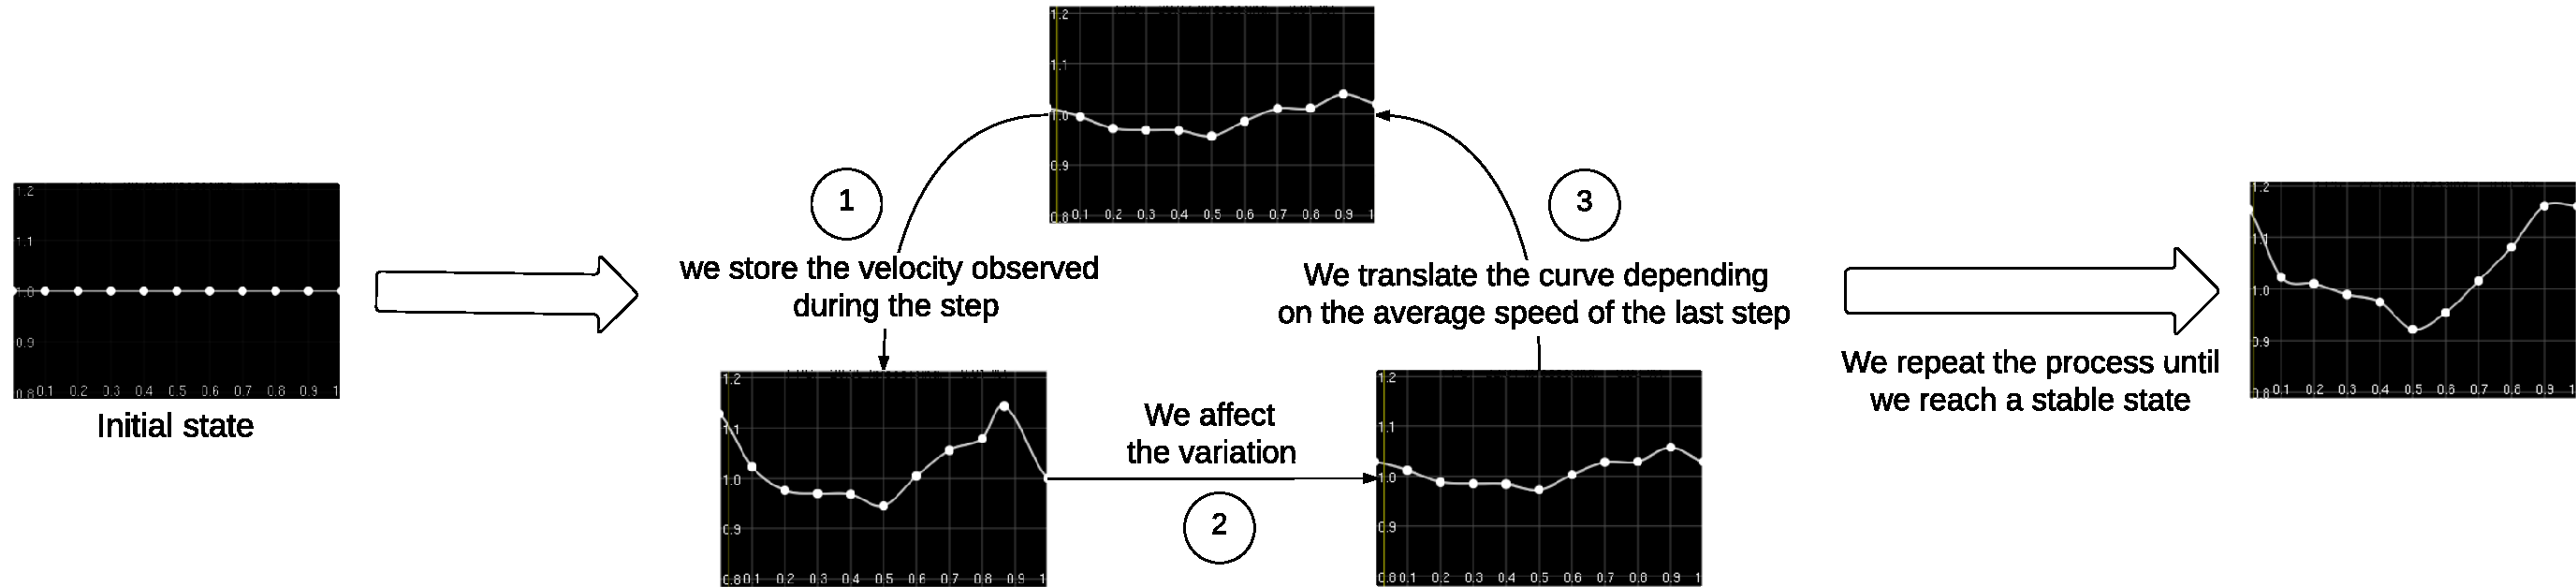
\includegraphics[scale=0.35]{images/speed_curve_learner.pdf}
\caption{Process of learning the adapted required velicity curve}
\label{fig:speed_curve_learner}
\end{figure*}

Similarly to the velocity tuning in~\cite{coros2010generalized}, our controller applies a horizontal virtual force to obtain a fine control of the speed and balance. Our version presents three major differences. First, we do not consider the same chain of limbs. Instead of considering one chain that goes from the head to the stance foot we use two: one going from the pelvis to the stance foot and one made of the torso alone. This modification comes from two considerations. First, we do not consider the head in the top chain because we do not want the character to tilt the head to control its velocity. Second, we separate the torso from the lower body because we estimate that the main control strategy of the speed should be to simply tilt the torso and not to exert huge torques on the stance ankle. To do so, our Jacobian matrix takes into account the mass $M_i$ of each individual limb:
$$
J_n ^T (p)=\frac{1}{M}\sum_{\substack{0<i\leq n}} ((P_i(x,y,z)-P_{i-1}(x,y,z))*M_i)
$$
where $M$ is the sum of the limbs' mass considered in the velocity tuning, $P_i(x,y,z)$ the position of the $i$ joint and $P_0(x,y,z)$ the application point of the virtual force. This modification allows us to give more importance to the joints controlling a lot of mass (i.e. the joint between the pelvis and the torso).

We also consider the intra-step velocity variations. In most cases, the velocity is not constant during a step. In most gait styles the character is faster at the start and end of a step than near the middle of it. Supposing it constant as in~\cite{coros2010generalized} may cause the apparition of undesired behaviors where the controller requests the character to slow down at the start of the step, then speed up near the middle of it, and to slow down once again at foot strike. To limit this issue, we use a system to learn the desired velocity at each instant of a step that is needed to produce a virtual force as constant as possible. This constant virtual force would result in the character moving at the global desired velocity. The \textit{learning velocity curve} is defined by $k$ key points uniformly distributed. The values between those points are computed using Catmull-Rom splines. Our tests have shown that a value of $k=11$ gives enough precision without being too time consuming.
The learning method is based on an iterative principle (see figure~\ref{fig:speed_curve_learner}). During a step we record the velocity of the center of mass of the character. When the step ends, we check if the average variation $\Delta_{avg}$ between the learning velocity curve and the velocity curve observed during the step $f_{obs}$ is lower than a threshold. If it is, we move each reference point of the learning velocity curve toward the values read in the observed velocity curve. To help converging without oscillations, we limit the maximum variation that can be affected to each key point to the average variation $\Delta_{avg}$. Then we adapt the learning curve so that it produces the user's desired speed. For the sagittal velocity, this adaptation is implemented as the scaling of the key points by the ratio $R_{sag}=V_d/V_{avg}$ between the desired velocity and the average observed velocity. For the coronal velocity, the adaptation is implemented as the translation of the key points by the difference $R_{cor}=V_d - V_{avg}$ between the desired velocity and the average observed velocity. So, at the end of the step $s$, each key point $f_s(i)$ is computed with the following equation  (the multiplication by $R_{sag}$ become an addition by $R_{cor}$ for the coronal curves):
\begin{equation}
f_s(i)= (f_{s-1}(i) + min(\Delta_{avg},f_{obs}(i)- f_{s-1}(i))) \times R_{sag}
\end{equation}
If the average variation $\Delta_{avg}$ is above the threshold it means the character is not in a stable motion anymore.
In that case we stop adapting our learning curve and switch to the use of recovery steps. This means the controller will now ignore the user specified swing foot trajectory and use the trajectory defined by the IPM for the totality of the step. The controller stays in recovery mode until the average variation between the observed speed and the specified one is lower than the threshold. If it takes more than five steps we reset the learning curve to the constant desired value and we start learning again. 

\section{Offline Optimization}
\label{sec:optimisation}

The goal of the offline optimization is to find the optimal parameters of our controller for a given scenario (desired character's speed and liquid height). The considered parameters are the swing foot trajectory and the coronal component of the angular trajectory for the following joints:
\begin{itemize}[noitemsep,nolistsep]
\item pelvis (3 trajectory key points)
\item joint between the pelvis and the torso (2 trajectory key points)
\item stance ankle (11 trajectory key points )
\item swing ankle (11 trajectory key points)
\item stance knee (5 trajectory key points)
\end{itemize}
The swing foot trajectory is defined by respectively 3, 5 and 11 key points for the x, y and z axis. So our optimization considers a total of 51 variables.

\subsection{Objective function}
During our optimization we use the following evaluation function:
\begin{equation}
\begin{split}
f_{eval} &=\sum_{\substack{t<k}} (\eta f_{energ} + \beta f_{drag} + \gamma f_{acc})\, *\\&(1+0.1* R_{ipm\_alt}) 
+ f_{speed} + f_{balance}
\label{eq:complete_eval}
\end{split}
\end{equation}
where $k$ is the duration in second of the evaluation. This function can be separated in two parts, each one composed of three functions. The first part corresponds to the sum and defines the characteristics of the motion that we want to observe once the optimization is complete. To do so we use a weighted sum of three functions, each one defining a specific behavior:
\begin{itemize}
\item{\textit{Minimization of consumed energy} ($f_{energ}$). The goal of this function is to obtain a motion using the minimum energy possible. This property is measured by the sum of the torques at every joint: $f_{energ}=\sum_{\substack{i}}{\tau_i}$} 
\item{\textit{Minimization of the drag}. ($f_{drag}$). Using this function, the character tries to move out of the liquid and it prevents velocity spikes within the liquid. We evaluate this property by using the sum of the torques induced by the drag forces on the parent joint of the limb where the drag forces $F_j$ are applied: $f_{energ}=\sum_{\substack{i}}\sum_{\substack{j}}((P_j(x,y,z)-P_i(x,y,z)) \times F_j)$ with  $P_j(x,y,z)$ the force application point and $P_i(x,y,z)$ the position of the parent joint.}
\item{\textit{Minimization of angular acceleration} ($f_{acc}$). The goal of this function is to obtain smooth motions that is measured by the sum of the angular accelerations in the reference poses $\ddot{\theta_d}_i$ and in the resulting motion $\ddot{\theta}_i$. We use a two coefficients to favor minimizing the accelerations of the actual motion: $f_{acc}=0.25*\sum_{\substack{i}}\ddot{\theta_d}_i+0.75*\sum_{\substack{i}}\ddot{\theta}_i$ }
\end{itemize}

The second part of the evaluation function consists of functions limiting the search space:
\begin{itemize}
\item{\textit{Penalization of IPM alteration} ($R_{ipm\_alt}$). The IPM alteration system is of great influence on the resulting motion. Even with reference poses defined to walk backward our system could succeed in walking forward if asked. To prevent this kind of situations, we penalize simulations heavily relying on the IPM alterations. To do so, we use the ratio between the IPM alteration required to obtain a stable motion ($\Delta(x,z)$) and its maximum threshold $max(\Delta(x,z))$ (0.09 in our tests): $R_{ipm\_alt}=\frac{\Delta(x,z)}{max(\Delta(x,z))}$}
\item{\textit{Velocity tracking} ($f_{speed}$). The goal of this function is to eliminate the simulations where the convergence to the desired velocity takes some time due to unsuitable reference trajectories. We use a high penalization value if the error on the velocity tracking is superior to 1\% of the desired velocity: if $||V-V_d||>0.01*||V_d||$ then $f_{speed}=10^{10}$}
\item{\textit{Motion balance} ($f_{balance}$). With this function, we verify if we have a stable motion by refusing simulations using recovery steps. If the system uses at least one recovery step, a high penalization value is given: $f_{balance}=10^{15}$}
\end{itemize}

\subsection{Optimization strategy}
Our fitness landscape presents many local minimums. As several physics-based animation systems~\cite{geijtenbeek2012simple,tan2011articulated}, we use a Covariance Matrix Adaptation (CMA)~\cite{hansen2006cma} to explore it.


\section{Implementation}
\label{sec:implementation}
The physics engine used is Open Dynamics Engine (ODE). The simulation step size is $5 \times 10^{-4}s$. The human model used is composed of 28 degrees of freedom, see \cite{coros2009robust} for more details. Collisions between the character's limbs are not considered. The gains of the PD-controller are kept constant through the simulation, and are the same as in the forward walking controller of~\cite{coros2009robust}. Joint torques are limited to $|\tau|<200Nm$  for the hips and knees and $|\tau|<100Nm$  for the other joints. The simulations are performed with a single-thread implementation on a common laptop with 8GB RAM and a 2.5GHz i5 processor. The controller proposed in this section as been build using a liquid with characteristics similar to water: $\rho=1000kg.m^{-3}$ and $\mu=1$.


\section{Results}
\label{sec:results}
All the results are best seen in the accompanying video.

\subsection{Offline Optimization}
First we studied the impact of the three minimization functions:
\begin{itemize}
\item\begin{minipage}[t]{\linewidth}{
The \textit{minimization of consumed energy} leads to steps keeping the swing foot near the ground in absence of water. When partially immersed, the character keeps the swing foot low but elevates it a bit higher to align the foot with the direction of the foot's velocity.}
\end{minipage}
\item\begin{minipage}[t]{\linewidth}{
The \textit{minimization of the liquid drag} leads to motions keeping the foot outside the water as long as possible until the water height is too high to do so (the limit is a bit above 0.5m which correspond to the knee height). It is interesting to note that the character uses a lateral movement to get the foot out of the water as fast as possible but it does strike as natural looking.}
\end{minipage}
\item\begin{minipage}[t]{\linewidth}{
The \textit{minimization of angular accelerations} leads to smooth motions keeping the swing foot near the ground with any water height but which prevents the character to recover from external pushes.}
\end{minipage}
\end{itemize}
We have chosen to use the weights $\eta=3$, $\beta=6$ and $\gamma=1$ for the evaluation function used to build our final controller. This combination leads to motions significantly influenced by the water height while keeping a natural looking movement. We also tried two others set of weights: 2,8,1 and 4,5,1. The fist of the two provoqued the apparition of the unnatural lateral displacement of the swingfoot we could observe when analysing the drag criteria. The second leaded to a movement that would choose to stay underwater even when water level was still under the knee.
With this objective function we have created 10 reference controllers. We have two sets of reference controllers corresponding to the character's speeds $0.3m.s^{-1}$ and $0.7m.s^{-1}$. Each set contains one controller for each of the five following water heights: 0, 0.25, 0.5, 0.75 and 1 meter.

\subsection{Final Controller}
\begin{figure}[t]
\centering
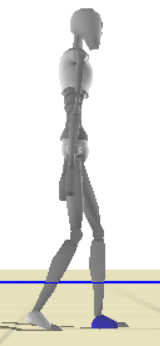
\includegraphics[scale=0.17]{images/strips/0_25/1.png}
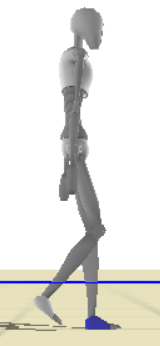
\includegraphics[scale=0.17]{images/strips/0_25/2.png}
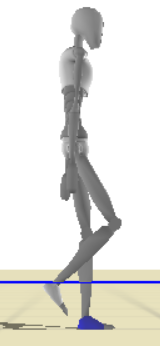
\includegraphics[scale=0.17]{images/strips/0_25/3.png}
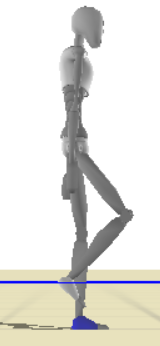
\includegraphics[scale=0.17]{images/strips/0_25/4.png}
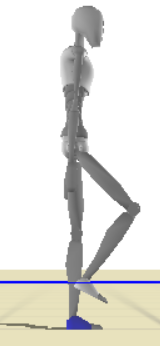
\includegraphics[scale=0.17]{images/strips/0_25/5.png}
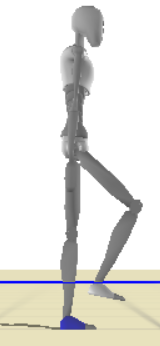
\includegraphics[scale=0.17]{images/strips/0_25/6.png}
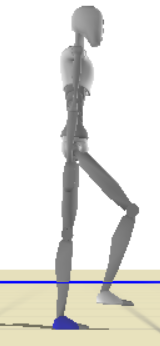
\includegraphics[scale=0.17]{images/strips/0_25/7.png}
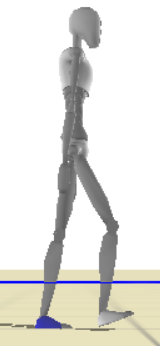
\includegraphics[scale=0.17]{images/strips/0_25/8.png}

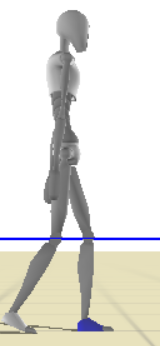
\includegraphics[scale=0.17]{images/strips/0_5/1.png}
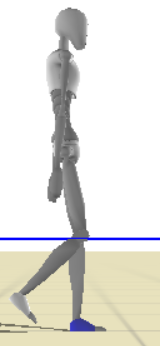
\includegraphics[scale=0.17]{images/strips/0_5/2.png}
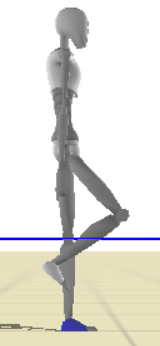
\includegraphics[scale=0.17]{images/strips/0_5/3.png}
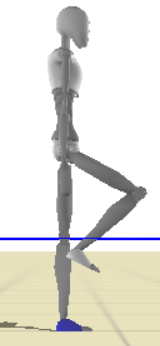
\includegraphics[scale=0.17]{images/strips/0_5/4.png}
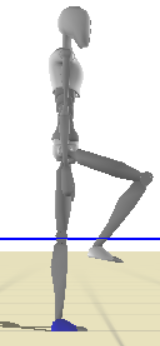
\includegraphics[scale=0.17]{images/strips/0_5/5.png}
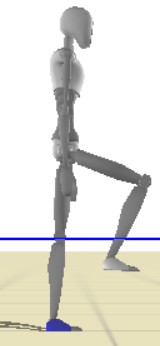
\includegraphics[scale=0.17]{images/strips/0_5/6.png}
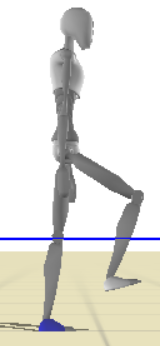
\includegraphics[scale=0.17]{images/strips/0_5/7.png}
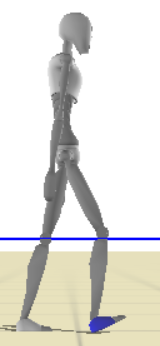
\includegraphics[scale=0.17]{images/strips/0_5/8.png}

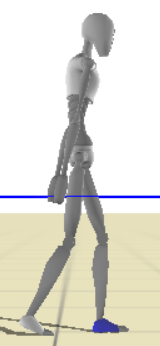
\includegraphics[scale=0.17]{images/strips/0_75/1.png}
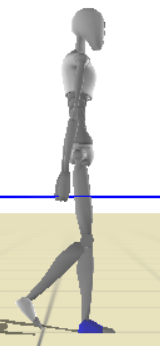
\includegraphics[scale=0.17]{images/strips/0_75/2.png}
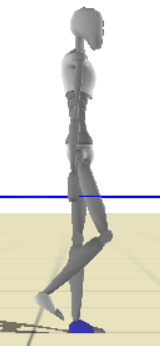
\includegraphics[scale=0.17]{images/strips/0_75/3.png}
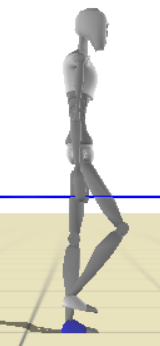
\includegraphics[scale=0.17]{images/strips/0_75/4.png}
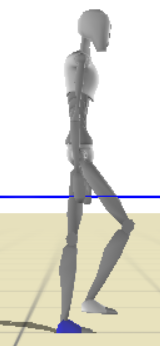
\includegraphics[scale=0.17]{images/strips/0_75/5.png}
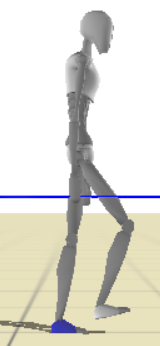
\includegraphics[scale=0.17]{images/strips/0_75/6.png}
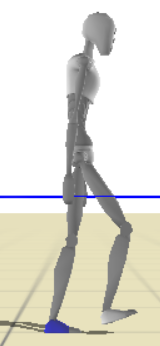
\includegraphics[scale=0.17]{images/strips/0_75/7.png}
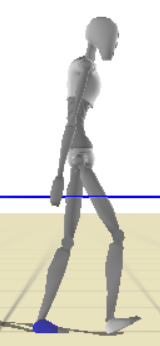
\includegraphics[scale=0.17]{images/strips/0_75/8.png}

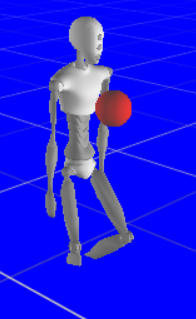
\includegraphics[scale=0.28]{images/strips/ball/img_impact.png}
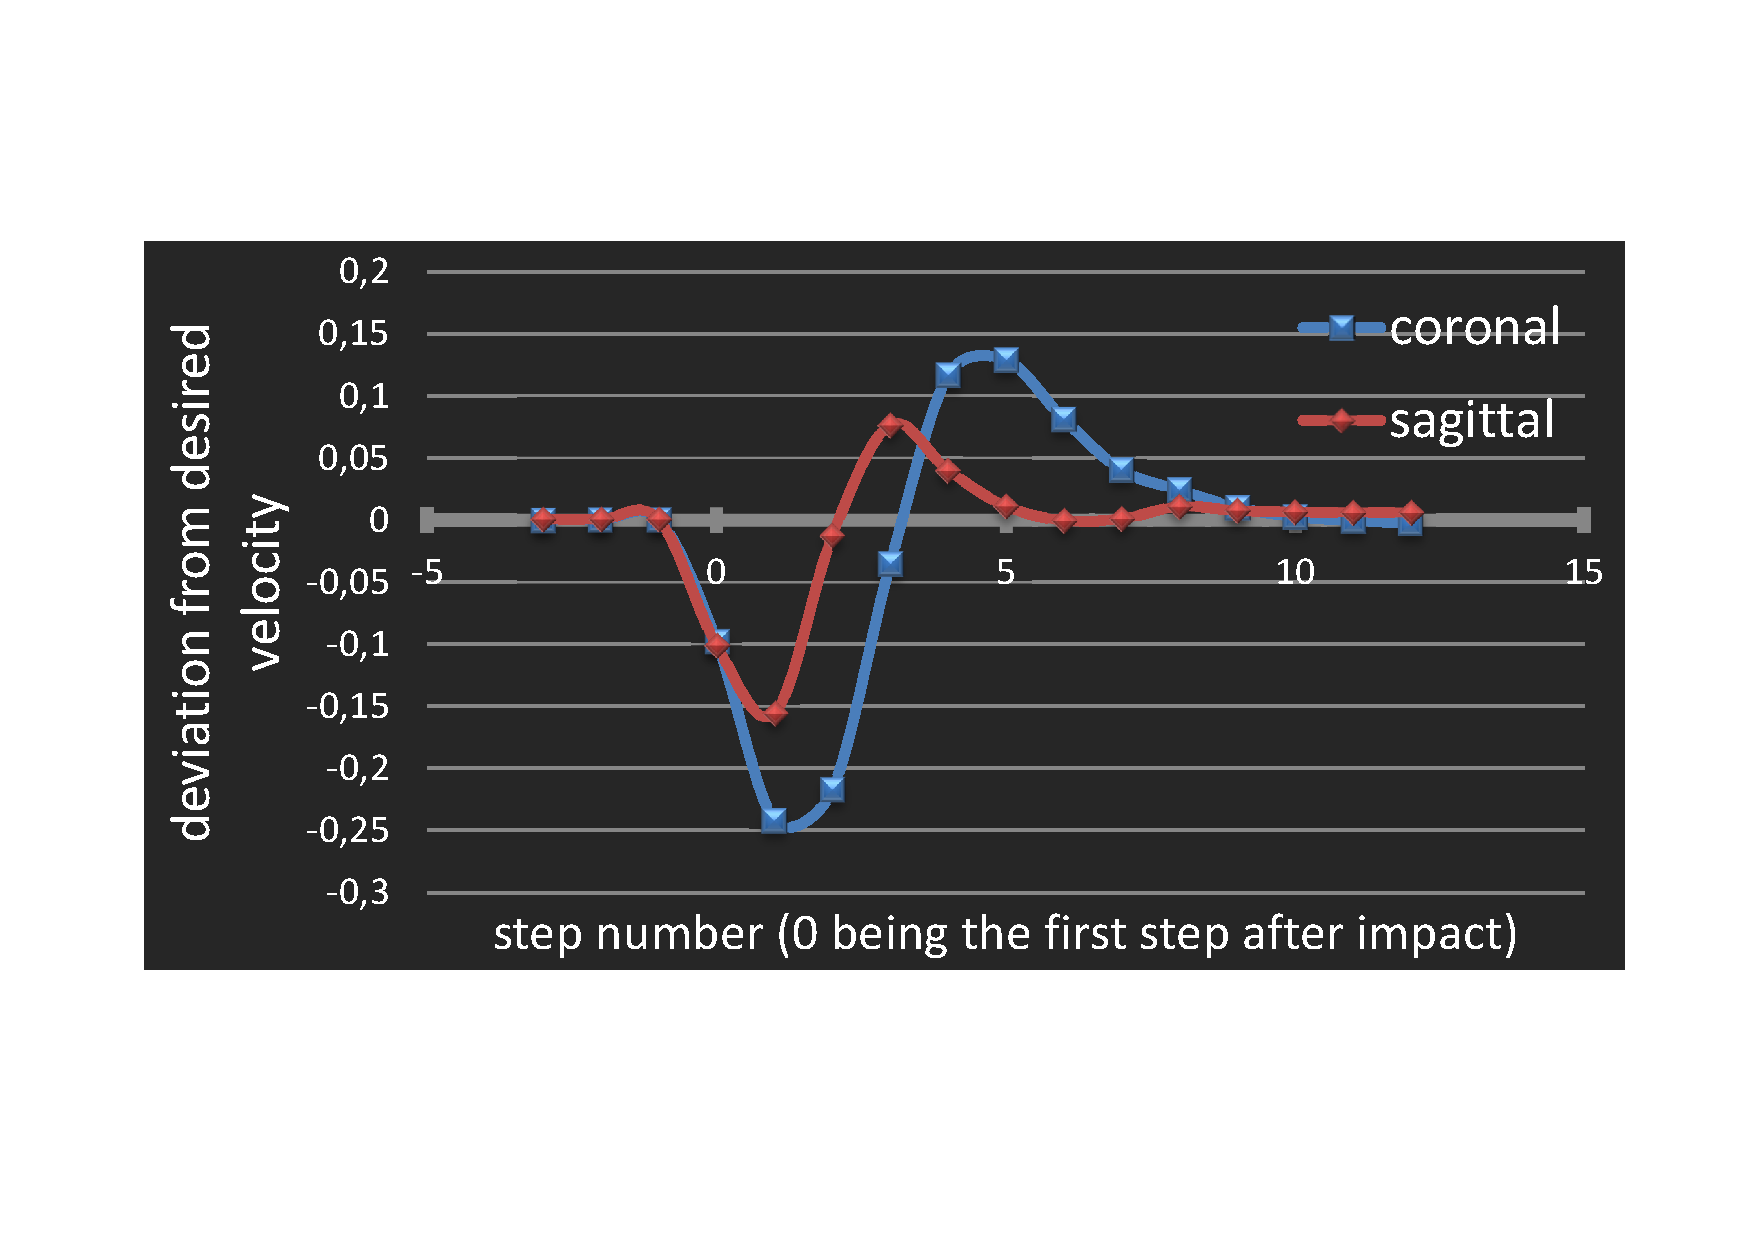
\includegraphics[scale=0.255]{images/strips/ball/speed_evo_after_impact.pdf}
\caption{Results obtained with our final controller. From top to bottom: character walking in 25cm, 50cm and 75cm of water. Bottom: character recovering from an external push, left: impact image, right: curves for the velocity deviation from the desired velocity. The character is moving at $0.6m.s{-1}$ in all the presented situations with no coronal speed.}
\label{fig:controller_results}
\end{figure}

Our controller allows online modification of the character's desired velocity. It is also possible to change the step width during movement. The controller is able to adapt to water height (figure~\ref{fig:controller_results}) as well as changes to the liquid's physics properties (density and viscosity). Our system is able to withstand external forces simulated through solid balls of 5kg projected onto the character (figure~\ref{fig:controller_results} bottom). All the simulations respect the real-time condition with a minimum of 27 fps when the water reachs the hips.
Our controller can reach any desired sagittal speed going from $0.2m.s{-1}$ to $0.7m.s{-1}$ uner any immertion heigh. The range of corronal speed that can be achieved goes from $-0.3m.s{-1}$ to $0.3m.s{-1}$.
The figure~\ref{fig:controller_results} illustrate some of the results. The first two rows of image show that the character adapts the height of the swing foot to reach the water height (first two rows). the third row illustrate the case where the water height is too high and the character keep the swing foot near the ground. The bottom row illustrate the character's recovery after an impact from a $5kg$ ball moving at $5.4m.s^{-1}$. As we can see, numerous steps are necessary to recover to a stable velocity.

\subsection{Limitations}

While our method to simulate the liquid allows real-time simulation, our implementation of the form drag stays an approximation of the real interactions and might lead to unrealistic results. The main problem with this limit is that even with our simplified implementation of the liquid impact our controller barely reach the 30fps, meaning that it would be difficult to find a way to simulate the liquid while keeping real-time animation. Our system cannot handle variations of the liquid viscosity five times superior to water viscosity, i.e. $\mu>5.0$, which is possibly caused by the previous limitation. Our system uses a static threshold to detect the need for recovery steps instead of using an adaptive value depending on if the velocity learning has been completed or not. We do not actively control the contact between the stance foot and the ground resulting in unstable foot ontrol expecialy when recovering from external pushes. This problem could be solved by adding a local feedback controller on the stance ankle. We have not demonstrated backward walk or in place walk but those motion should be possible as long as the simple controllers defining their differences with the forward walk are added. Our system presents some difficulty to reach the desired coronal velocities expecialy if the variation desired is sudden. This is most likely cause by the fact that we need two learning velocity curves for the coronal axis. Adding a learning system with direct impact of the evolution of one curve on the other could be a possible solution.
%*** + limitations par rapport à la densité, la hauteur d'eau, le respect de la vitesse, les forces externes, l'écartement des pas, etc. ***
%*** + proposer des améliorations et relativiser les limitations ***

\section{Conclusion}
\label{sec:conclusion}

We have presented a physics-based controller capable of real-time interactive simulation of walking motions for partially immersed bipeds. We have demonstrated online adaptation of the gait style to external conditions such as the liquid height and desired character's speed. Our controller permits the specification of new gait styles specific to walking motions in a liquid medium.

Our controller could be extended by implementing a more realistic liquid model which would consider the perturbations of the liquid caused by the character. Adding other mediums (e.g. snow-like mediums) or movement types (e.g. standing still, running…) with possible online transition between them are also interesting works we would like to investigate.
%*** en dire plus ***

%\section*{Acknowledgements}

%\nocite{*}
\bibliographystyle{acmsiggraph}
\bibliography{template}
\end{document}
